\documentclass{article}
\usepackage{amsmath}
\usepackage{amsfonts}
\usepackage{amssymb}
\usepackage{tcolorbox}
\usepackage[inline]{enumitem}
\usepackage[a4paper,margin=1in]{geometry}
\usepackage[normalem]{ulem}
\usepackage{graphicx}
\usepackage{tasks}
\settasks{label=(\alph*), label-offset=0.4em, label-width=1.5em}

\usepackage{fancyhdr}
\fancyhf{}
\setlength{\headheight}{36pt}
\renewcommand{\headrulewidth}{0pt}
\thispagestyle{fancy}
\lhead{Calculus Exercise}
\chead{Week 9 (5.1, 5.2, 5.3)}
\rhead{\underline{ID:\hspace{7.4em}} \\ \vspace{0.2cm} \underline{Name:\hspace{6em}}}
\cfoot{\thepage}

\begin{document}
\begin{enumerate}
\item[5.1.18]
    Use the following \textbf{Definition} to find an expression for
    the area under the graph $f(x) = x + \ln x,\ 3 \leqslant x \leqslant 8$
    as a limit. You don't need to evaluate the limit.

    \begin{tcolorbox}
        \textbf{Definition.} The \textbf{area} $A$ of the region
        $\displaystyle S = \bigcup_{k=1}^{n} S_{n}$
        that lies under the graph of the continuous function $f$
        on the interval $[a, b]$ is the limit of the sum of the
        areas of approximating rectangles:
        \[
            A = \lim_{n \to \infty} \sum_{k=1}^{n} f(x_{k}) \Delta x
            ,\ \Delta x = x_1 - a = b - x_{n-1} = x_{i} - x_{i-1} \text{ for } 1 \leqslant i \leqslant n.
        \]

        \begin{center}
            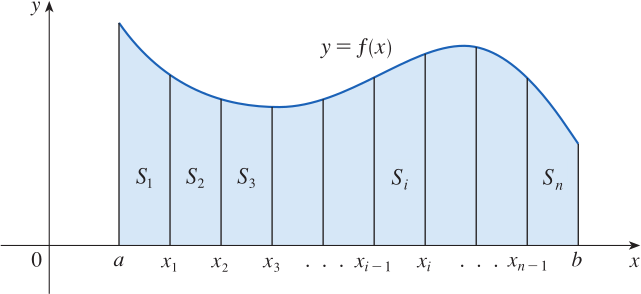
\includegraphics[width=8cm]{./png/5.1.18.png}
        \end{center}
    \end{tcolorbox}

\vspace{7cm}

\item[5.1.22]
    Determine a region whose area is equal to the given limit.
    You don't need to evaluate the limit.
    \[
        \lim_{n \to \infty} \sum_{i=1}^{n} \frac{3}{n}\sqrt{1 + \frac{3i}{n}}
    \]

\newpage

\item[5.1.34]
    \begin{enumerate}
        \item
            Let $A_{n}$ be the area of a polygon with $n$ equal sides
            inscribed in a circle with radius $r$. By dividing,
            the polygon into $n$ congruent triangles with central angle $2 \pi / n$,
            show that
            \[
                A_{n} = \frac{1}{2}n r^{2} \sin \left(\frac{2 \pi }{n}\right)
            \]
        \item
            Show that
            \[
                \lim_{n \to \infty} A_{n} = \pi r^{2}.
            \]
    \end{enumerate}

\vspace{6cm}

\item[5.2.23]
    Show that the definite integral is equal to $\displaystyle  \lim_{n \to \infty} R_{n}$,
    and then evaluate the limit.
    \[
        \int_{0}^{4} (x - x^{2}) dx,\ R_{n} =
        \frac{4}{n} \sum_{i=1}^{n} \left( \frac{4i}{n} - \frac{16i^{2}}{n^{2}} \right)
    \]

\vspace{6cm}

\item[5.2.57]
    Write as a single integral in the form $\displaystyle \int_{a}^{b} f(x) dx$:
    \[
        \int_{-2}^{2} f(x) dx + \int_{2}^{5} f(x) dx - \int_{-2}^{-1} f(x)dx
    \]

\newpage

\item[5.2.60]
    Find $\displaystyle \int_{0}^{5} f(x) dx$ if
    \[
        f(x) =
        \begin{cases}
            3&,\ x < 3\\
            x&,\ x \geqslant 3
        \end{cases}
    \]

\vspace{5cm}

\item[5.2.68]
    Use the properties of integrals to verify the inequality without evaluating the integrals.
    \[
        \frac{\pi}{12} \leqslant \int_{\frac{\pi}{6}}^{\frac{\pi}{3}} \sin x dx
        \leqslant \frac{\sqrt{3} \pi }{12}
    \]

\vspace{5cm}

\item[5.3.58]
    Sketch the region enclosed by the given curves and calculate its area.
    \[
        y = 2x - x^{2},\ y = 0
    \]

\newpage

\item[5.3.68]
    Find the derivative of the function.
    \[
        g(x) = \int_{1-2x}^{1+2x} t \sin t dt
    \]

\vspace{4cm}


\item[5.3.76]
    If $\displaystyle f(x) = \int_{0}^{\sin x} \sqrt{1+t^{2}} dt$ and
    $\displaystyle  g(y) = \int_{3}^{y} f(x) dx$,
    find $g''(\frac{\pi}{6})$.

\vspace{4cm}

\item[5.3.78]
    Use l'Hospital's Rule to evaluate the limit.
    \[
        \lim_{x \to \infty} \frac{1}{x^{2}} \int_{0}^{x} \ln(1 + e^{t}) dt
    \]

\vspace{4cm}

\item[5.3.93]
    Find a function $f$ and a number $a$ such that
    \[
        6 + \int_{a}^{x} \frac{f(t)}{t^{2}}dt = 2 \sqrt{x},\ \forall\ x > 0.
    \]
\end{enumerate}
\end{document}
